\documentclass[12pt,a4paper]{article}

% Paquetes básicos
\usepackage[utf8]{inputenc}
\usepackage[T1]{fontenc}
\usepackage[spanish]{babel}
\usepackage{amsmath, amssymb}
\usepackage{siunitx} % Ángulos
\usepackage{graphicx}
\usepackage{float}
\usepackage{geometry}
\geometry{margin=2.5cm}
\usepackage{hyperref}
\usepackage{caption}
\usepackage{subcaption}
\usepackage{setspace}
\usepackage{multirow}

\usepackage{listings}
\usepackage{xcolor}

\lstdefinestyle{matlab}{
    language=Matlab,
    backgroundcolor=\color{gray!10},
    basicstyle=\ttfamily\small,
    keywordstyle=\color{blue}\bfseries,
    commentstyle=\color{green!50!black},
    stringstyle=\color{red},
    numbers=left,
    numberstyle=\tiny\color{gray},
    stepnumber=1,
    numbersep=8pt,
    tabsize=4,
    breaklines=true,
    showstringspaces=false,
}
\onehalfspacing


% Datos
\author{Nombre y Apellido \\ Legajo: XXXXX}
\date{\today}

\begin{document}

% Carátula personalizada
\begin{titlepage}
    \centering
    
\includegraphics[width=0.25\textwidth]{escudo.png} 
    \hspace{1cm}
    
\includegraphics[width=0.3\textwidth]{download.png} \\[1cm]

    {\large \textbf{UNIVERSIDAD NACIONAL DE CÓRDOBA} \\[0.5cm]}
    {\large \textbf {FACULTAD DE CIENCIAS EXACTAS, FÍSICAS Y NATURALES} \\[1cm]}
    {\Large SÍNTESIS DE REDES ACTIVAS \\[1cm]}

    \rule{\textwidth}{0.5pt} \\[0.5cm]
    {\Large \textbf{Trabajo Práctico N°4} \\[0.3cm]}
    {\Large \textbf{Filtros Activos} \\[0.3cm]}
    \rule{\textwidth}{0.5pt} \\[1cm]

\begin{tabular}{l l}
\textbf{Profesor Titular:} & Dr. Ing. Ferreyra Pablo \\
\textbf{Profesor Adjunto:} & Ing. Reale Cesar \\
\\
\textbf{Alumnos:} & Dávila Tomassi, Carlos Valentino \\
 & Mendes Rosa, Agustín \\
 & Monja, Ernesto Joaquín \\
\end{tabular}\\[3cm]

{\centering Año 2025 \par}

\end{titlepage}



% Índice
\tableofcontents
\newpage
\indent



\section{Introducción}
\subsection{Consigna}
En este trabajo práctico, se busco sintetizar un filtro pasa banda de acuerdo a los requerimientos presentados en la siguiente figura
\begin{figure}[H]
    \centering
    
\includegraphics[width=1\textwidth]{Figura 1.png}
    \caption{Requerimientos del Filtro Pasa Banda.} 
\end{figure}

De esta imagen, se pueden listar que las especificaciones de este filtro son las siguientes:
\begin{itemize}
    \item \underline{Banda de Paso:} $f_p = 800 \ a \ 1250 \ [Hz]$
    \item \underline{Banda de Rechazo:} $f_a = 0 \ a \ 200 \ [Hz] \ y \ 5000 \ a \ \infty \ [Hz]$
    \item \underline{Atenuación Máxima en la Banda de Paso:} $A_{max}= 0,25 \ [dB]$
    \item \underline{Atenuación Mínima en la Banda de Rechazo:} $A_{min} = 30 \ [dB]$
\end{itemize}

Con estos requerimientos listados, procedemos en las secciones posteriores al diseño de un filtro que cumpla con estas especificaciones utilizando la bibliografía referenciada en clase.



\section{Desarrollo}
\subsection{Aproximación de la función de atenuación mediante Matlab}
Se tiene que los parámetros descritos en la sección precedente deben formar una función de transferencia la cual aproximaremos mediante polinomios de Chebyshev con Matlab. Utilizando las funciones cheb1ord y cheby1 de Matlab según el código adjunto en el Anexo 1, se deduce que el filtro deberá tener una función de transferencia tal como la que se muestra a continuación: 
\begin{equation}
    \label{eq_1}
    T(s)= \frac{1,642x10^7 s^2}{s^4 + 5080 s^3 + 9,586x10^7 s^2 + 2,006x10^{11} s + 1,559x10^{15}}
\end{equation}

De aquí, podemos hacer uso de la aproximación en cascada de 2 funciones de transferencia canónicas y bicuadráticas. Esto quiere decir que nuestro filtro pasa banda estará compuesto por un filtro Pasa Bajos en cascada con un Pasa Altos los cuales en conjunto conformarán el Pasa Banda con las especificaciones listadas. El código utilizado de Matlab ya incluye una descomposición bicuadrática de estos filtros de modo tal que las funciones de estos filtros son:

\begin{equation}
    \label{eq_2}
    T_{PB} = \frac{3,284x10^{7}}{s^2 + 3184s + 6,632x10^{7}}
\end{equation}

\begin{equation}
    \label{eq_3}
    T_{PA} = \frac{0,5s^{2}}{s^2 + 1896s + 2,35x10^{7}}
\end{equation}

A continuación se presenta un diagrama de bode tanto del filtro completo como del accionar de cada una de sus bicuadráticas:

\begin{figure}[H]
    \centering
    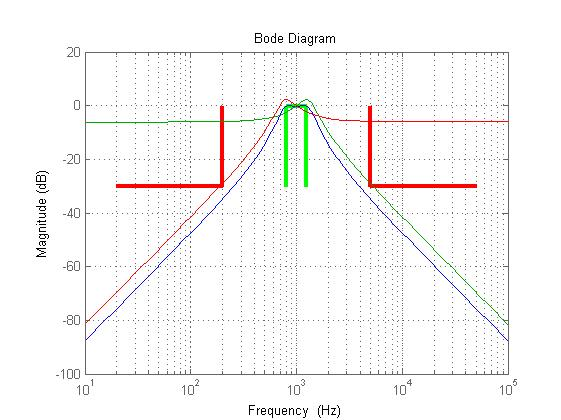
\includegraphics[width=0.7\linewidth]{Figura 2.jpg}
    \caption{Diagrama de Bode del Filtro Pasa Banda.}
\end{figure}



\subsection{Síntesis de los Filtros}
\subsubsection{Filtro Pasa Bajos}
El primer filtro que diseñaremos será el filtro Pasa Bajos el cual seguirá una topología de realimentación positiva y según la bibliografía, nos supone un circuito tal como el que se presenta en la siguiente figura:

\begin{figure}[H]
    \centering
    
\includegraphics[width=1\linewidth]{Figura 3.png}
    \caption{Filtro Pasa Bajos de Topología de Realimentación positiva.}
\end{figure}

Planteando las ecuaciones de nodos del sistema, se tiene que:

\begin{equation}
    \label{eq_4}
    (v_{x} - v_{in})\frac{1}{R_1} + (v_{x} - v_{o})sC_{1} + (v_{x} - v^{+})\frac{1}{R_{2}} = 0
\end{equation}
\begin{equation}
    \label{eq_5}
    (v^{+} - v_{x})\frac{1}{R_2} + v^{+}sC_2 = 0
\end{equation}

Agrupando términos se llega a:

\begin{equation}
    \label{eq_6}
    \left(\frac{1}{R_1} + \frac{1}{R_2} + sC_1\right)v_x + \left(-\frac{1}{R_2}\right)v^{+} = v_{in}\left(\frac{1}{R_1}\right) + v_{o}(sC_1)
\end{equation}
\begin{equation}
    \label{eq_7}
    \left(-\frac{1}{R_2}\right)v_x + \left(\frac{1}{R_2} + sC_2\right)v^{+} = 0
\end{equation}

Finalmente el sistema matricial es igual a:

\begin{equation}
    \label{eq_8}
    \begin{bmatrix}
        \frac{1}{R_1} + \frac{1}{R_2} + sC_1  & -\frac{1}{R_2} \\
        -\frac{1}{R_2} & \frac{1}{R_2} + sC_2    
    \end{bmatrix} . 
    \begin{bmatrix}
        v_x \\
        v^+
    \end{bmatrix} =
    \begin{bmatrix}
        sC_1 & \frac{1}{R_1} \\
        0 & 0
    \end{bmatrix} . 
    \begin{bmatrix}
        v_o \\
        v_{in}
    \end{bmatrix}
\end{equation}

Se puede resolver este sistema utilizando la resolución por Regla de Crammer, donde se definen para este circuito la Función de Transferencia de Realimentación ($T_{FB}$) y la función de Transferencia de Avance ($T_{FF}$) como:

\begin{equation}
    \label{eq_9}
    T_{FB} = \left(\frac{V_1}{V_3}\right)_{V_2 = 0} = \left(\frac{v^+}{v_{o}}\right)_{v_{in} = 0} = \frac{\frac{s}{R_{2}C_{2}}}{s^2 + s\left(\frac{1}{R_{1}C_{1}} + \frac{1}{R_{2}C_{1}} + \frac{1}{R_{2}C_{2}}\right) + \frac{1}{R_{1}R_{2}C_{1}C_{2}}}= \frac{N_{FB}}{D_{FB}}
\end{equation}

\begin{equation}
    \label{eq_10}
    T_{FF} = \left(\frac{V_1}{V_2}\right)_{V_3 = 0} = \left(\frac{v^+}{v_{in}}\right)_{v_{o} = 0} = \frac{\frac{1}{R_{1}R_{2}C_{1}C_{2}}}{s^2 + s\left(\frac{1}{R_{1}C_{1}} + \frac{1}{R_{2}C_{1}} + \frac{1}{R_{2}C_{2}}\right) + \frac{1}{R_{1}R_{2}C_{1}C_{2}}} = \frac{N_{FF}}{D_{FF}}
\end{equation}

Nótese que dada la resolución por Regla de Crammer, se tiene que el denominador de las funciones de transferencia de $T_{FB}$ y $T_{FF}$ son iguales es decir que: $D_{FB} = D_{FF} = D$, mientras que los  numeradores son distintos, es decir: $N_{FB} \ne N_{FF}$. Por este motivo, podemos plantear que la Función de Transferencia de la Topología de Realimentación Positiva será igual a:

\begin{equation}
    \label{eq_11}
    T_V = \frac{v_{o}}{v_{in}} = \frac{k N_{FF}}{D - kN_{FB}}
\end{equation}

Donde $k$ es la ganancia de lazo cerrado ideal dada por la realimentación negativa, la cual se debe definir como: 

\begin{equation}
    \label{eq_12}
    k = 1 + \frac{r_{2}}{r_{1}}
\end{equation}

Reemplazando los numeradores de (\ref{eq_9}) y (\ref{eq_10}) en (\ref{eq_11}), se llega a que:

\begin{equation}
    \label{eq_13}
    T_V = \frac{\frac{k^2}{R_{1}R_{2}C_{1}C_{2}}}{s^2 + s\left(\frac{1}{R_{1}C_{1}} + \frac{1}{R_{2}C_{1}} + \frac{1-k}{R_{2}C_{2}}\right) + \frac{1}{R_{1}R_{2}C_{1}C_{2}}}
\end{equation}

Luego, sabemos que esa expresión debería ser igual termino a termino a la expresión encontrada para el Filtro Pasa Bajo la cual sigue la expresión encontrada en (\ref{eq_2}), por lo que igualando termino a termino, se deduce que:

\begin{equation}
    \label{eq_14}
    \frac{k^2}{R_{1}R_{2}C_{1}C_{2}} = 3,284x10^{7}
\end{equation}
\begin{equation}
    \label{eq_15}
    \frac{1}{R_{1}R_{2}C_{1}C_{2}} = 6,632x10^{7}
\end{equation}
\begin{equation}
    \label{eq_16}
    \frac{1}{R_{1}C_{1}} + \frac{1}{R_{2}C_{1}} + \frac{1-k}{R_{2}C_{2}} = 3184
\end{equation}

Nótese que se tienen mas incógnitas que ecuaciones en las ultimas 3 planteadas, por lo tanto deberemos fijar nosotros, bajo un criterio razonable, que incógnitas fijamos. Se elije entonces que:

\begin{itemize}
    \item $C_{1} = C_{2} = 47 \ [nF]$
    \item $R_{1} = R_{2} = R$ 
\end{itemize}

Se igualaron los capacitores a $47 \ [nF]$ debido a que este es un valor comercial fácilmente accesible para diseñar y armar este filtro, mientras que las resistencias se igualaron para permitir obtener una solución única. Con estas consideraciones en mente, resulta que las ecuaciones (\ref{eq_14}), (\ref{eq_15}) y (\ref{eq_16}) se simplifican a:

\begin{equation}
    \label{eq_17}
    \frac{k^2}{R^{2}C^{2}} = 3,284x10^{7}
\end{equation}
\begin{equation}
    \label{eq_18}
    \frac{1}{R^{2}C^{2}} = 6,632x10^{7}
\end{equation}
\begin{equation}
    \label{eq_19}
    \frac{3-k}{RC} = 3184
\end{equation}

Si $C = 47 \ [nF]$, podemos despejar $R$ de la ecuación (\ref{eq_18}), tal que:

\begin{equation}
    \label{eq_20}
    R = \sqrt{\frac{1}{6,632x10^{7} (47 \ [nF])^2}} = 2612,64 \ [\Omega]
\end{equation}

Luego, sabiendo $R$ y $C$, podemos despejar $k$ de la ecuación (\ref{eq_19}), tal que:

\begin{equation}
    \label{eq_21}
    3 - k = 3184(RC) 
\end{equation}
\begin{equation}
    \label{eq_22}
    k = 3 - 3184(2612,64)(47x10^{-9})
\end{equation}

Finalmente se deduce que: $k = 2,609$ de modo tal que siguiendo lo mencionado en (\ref{eq_12}), si fijamos a $r_2 = 20 \ [k \Omega]$ de modo tal que:

\begin{equation}
    \label{eq_23}
    r_1 = \frac{r_2}{k-1} = \frac{20000 \ [\Omega]}{2,609 - 1} = 12429,89\ [\Omega]
\end{equation}

Finalmente, se debe verificar que con los valores elegidos se cumpla la relación expuesta en (\ref{eq_17}) tal que:

\begin{equation}
    \label{eq_24}
    \left(\frac{2,609}{2612,64(47x10^{-9})}\right)^2 \approx 451,43x10^6
\end{equation}

Nótese que como el resultado obtenido en (\ref{eq_24}) es diferente al obtenido en (\ref{eq_17}), donde el primero es almenos 10 veces mayor al segundo, lo que implica que la ganancia del circuito es mucho mayor que la requerida por las especificaciones del circuito, por lo tanto se debe introducir una impedancia extra para reducir la ganancia, tal como muestra la siguiente figura:

\begin{figure}[H]
    \centering
    
\includegraphics[width=0.7\linewidth]{Figura 4.png}
    \caption{Ajuste de Ganancia con Impedancias de Entrada.}
\end{figure}

Se deduce entonces que la ganancia de la atenuación estará dada por:

\begin{equation}
    \label{eq_25}
    A_{atenuacion} = \frac{3,284x10^{7}}{451,43x10^6} \approx 0,0727
\end{equation}

De modo tal que los valores de las resistencias serán:

\begin{equation}
    \label{eq_26}
    R_1 = \frac{R}{A_{atenuacion}} = \frac{2612,64}{0,0727} \approx 35914,25 [\Omega]
\end{equation}

\begin{equation}
    \label{eq_27}
    R_1' = \frac{R}{1 - A_{atenuacion}} = \frac{2612,64}{1 - 0,0727} \approx 2817,47 [\Omega]
\end{equation}

Resulta entonces que ajustando estos valores de resistencias a sus valores comerciales, se obtiene el siguiente circuito:

\begin{figure}[H]
    \centering
    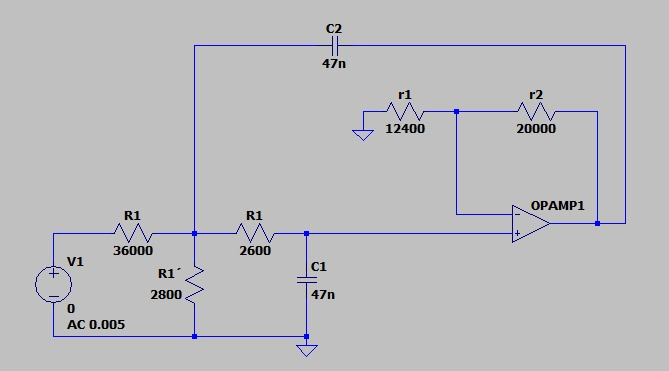
\includegraphics[width=0.8\linewidth]{Figura 5.jpg}
    \caption{Filtro Pasa Bajos Final.}
\end{figure}








\subsubsection{Filtro Pasa Altos}
El segundo filtro que diseñaremos será el filtro Pasa Altos el cual seguirá una topología de realimentación positiva y supone un circuito tal como el que se presenta en la siguiente figura:

\begin{figure}[H]
    \centering
    
\includegraphics[width=0.6\linewidth]{Figura 6.png}
    \caption{Filtro Pasa Altos de Topología de Realimentación positiva.}
\end{figure}

Planteando las ecuaciones de nodos del sistema, se tiene que:

\begin{equation}
    \label{eq_28}
    (v_{x} - v_{in})sC_{1} + (v_{x} - v_{o})\left(\frac{1}{R_{1}}\right) + (v_{x} - v^{+})sC_{2} = 0
\end{equation}
\begin{equation}
    \label{eq_29}
    (v^{+} - v_{x})sC_{2} + v^{+}\left(\frac{1}{R_{2}}\right) = 0
\end{equation}

Agrupando términos se llega a:

\begin{equation}
    \label{eq_30}
    \left(\frac{1}{R_{1}} + sC_{1} + sC_{2}\right)v_{x} + (-sC_{2})v^{+} = (sC_1)v_{in} + \left(\frac{1}{R_1}\right)v_{o}
\end{equation}
\begin{equation}
    \label{eq_31}
    (-sC_2)v_x + \left(\frac{1}{R_2} + sC_2\right)v^{+} = 0
\end{equation}

Finalmente el sistema matricial es igual a:

\begin{equation}
    \label{eq_32}
    \begin{bmatrix}
        \frac{1}{R_{1}} + sC_{1} + sC_{2}  & -sC_{2} \\
        -sC_{2} & \frac{1}{R_2} + sC_2    
    \end{bmatrix} . 
    \begin{bmatrix}
        v_x \\
        v^+
    \end{bmatrix} =
    \begin{bmatrix}
        sC_1 & \frac{1}{R_1} \\
        0 & 0
    \end{bmatrix} . 
    \begin{bmatrix}
        v_o \\
        v_{in}
    \end{bmatrix}
\end{equation}

Se puede resolver este sistema utilizando la resolución por Regla de Crammer, donde se definen para este circuito la Función de Transferencia de Realimentación ($T_{FB}$) y la función de Transferencia de Avance ($T_{FF}$) como:

\begin{equation}
    \label{eq_33}
    T_{FB} = \left(\frac{v^+}{v_{o}}\right)_{v_{in} = 0} = \frac{\frac{s}{R_{2}C_{2}}}{s^2 + s\left(\frac{1}{R_{1}C_{1}} + \frac{1}{R_{2}C_{1}} + \frac{1}{R_{2}C_{2}}\right) + \frac{1}{R_{1}R_{2}C_{1}C_{2}}}= \frac{N_{FB}}{D_{FB}}
\end{equation}

\begin{equation}
    \label{eq_34}
    T_{FF} = \left(\frac{v^+}{v_{in}}\right)_{v_{o} = 0} = \frac{s^2}{s^2 + s\left(\frac{1}{R_{1}C_{1}} + \frac{1}{R_{2}C_{1}} + \frac{1}{R_{2}C_{2}}\right) + \frac{1}{R_{1}R_{2}C_{1}C_{2}}} = \frac{N_{FF}}{D_{FF}}
\end{equation}

Nótese que dada la resolución por Regla de Crammer, se tiene que el denominador de las funciones de transferencia de $T_{FB}$ y $T_{FF}$ son iguales es decir que: $D_{FB} = D_{FF} = D$, mientras que los  numeradores son distintos, es decir: $N_{FB} \ne N_{FF}$. Por este motivo, podemos plantear que la Función de Transferencia de la Topología de Realimentación Positiva será igual a la expresión encontrada en (\ref{eq_11}), tal que reemplazando los numeradores de (\ref{eq_33}) y (\ref{eq_34}) en (\ref{eq_11}), se llega a que:

\begin{equation}
    \label{eq_35}
    T_V = \frac{ks^2}{s^2 + s\left(\frac{1}{R_{1}C_{1}} + \frac{1}{R_{2}C_{1}} + \frac{1-k}{R_{2}C_{2}}\right) + \frac{1}{R_{1}R_{2}C_{1}C_{2}}}
\end{equation}

Luego, sabemos que esa expresión debería ser igual termino a termino a la expresión encontrada para el Filtro Pasa Alto la cual sigue la expresión encontrada en (\ref{eq_3}), por lo que igualando termino a termino, se deduce que:

\begin{equation}
    \label{eq_36}
    k = 0,5
\end{equation}
\begin{equation}
    \label{eq_37}
    \frac{1}{R_{1}R_{2}C_{1}C_{2}} = 2,35x10^{7}
\end{equation}
\begin{equation}
    \label{eq_38}
    \frac{1}{R_{1}C_{1}} + \frac{1}{R_{2}C_{1}} + \frac{1-k}{R_{2}C_{2}} = 1896
\end{equation}

Nótese que se tienen mas incógnitas que ecuaciones en las ultimas 3 planteadas, por lo tanto deberemos fijar nosotros, bajo un criterio razonable, que incógnitas fijamos. Se elije entonces que:

\begin{itemize}
    \item $C_{1} = C_{2} = 47 \ [nF]$
    \item $R_{1} = R_{2} = R$ 
\end{itemize}

Se igualaron los capacitores a $47 \ [nF]$ debido a que este es un valor comercial fácilmente accesible para diseñar y armar este filtro, mientras que las resistencias se igualaron para permitir obtener una solución única. Con estas consideraciones en mente, resulta que las ecuaciones (\ref{eq_37}) y (\ref{eq_38}) se simplifican a:

\begin{equation}
    \label{eq_39}
    \frac{1}{R^{2}C^{2}} = 2,35x10^{7}
\end{equation}
\begin{equation}
    \label{eq_40}
    \frac{3-k}{RC} = 1896
\end{equation}

Si $C = 47 \ [nF]$, podemos despejar $R$ de la ecuación (\ref{eq_39}), tal que:

\begin{equation}
    \label{eq_41}
    R = \sqrt{\frac{1}{2,35x10^{7} (47 \ [nF])^2}} = 4389,02 \ [\Omega]
\end{equation}

Luego, sabiendo $R$ y $C$, podemos despejar $k$ de la ecuación (\ref{eq_40}), tal que:

\begin{equation}
    \label{eq_42}
    3 - k = 1896(RC)
\end{equation}
\begin{equation}
    \label{eq_43}
    k = 3 - 1896(4389,02)(47x10^{-9}) = 2,609
\end{equation}

De modo tal que siguiendo lo mencionado en (\ref{eq_12}), si fijamos a $r_2 = 20 \ [k \Omega]$ de modo tal que:

\begin{equation}
    \label{eq_44}
    r_1 = \frac{r_2}{k-1} = \frac{20000 \ [\Omega]}{2,609 - 1} = 12429,89\ [\Omega]
\end{equation}

Nótese que como el resultado obtenido en (\ref{eq_43}) es diferente al obtenido en (\ref{eq_36}), donde el primero es al menos 5 veces mayor al segundo, lo que implica que la ganancia del circuito es mucho mayor que la requerida por las especificaciones del circuito, por lo tanto se debe introducir una impedancia extra para reducir la ganancia, siguiendo lo mostrado en la Figura 4 donde se deduce que la ganancia de la atenuación estará dada por:

\begin{equation}
    \label{eq_45}
    A_{atenuacion} = \frac{0,5}{2,608} \approx 0,1916
\end{equation}

De modo tal que los valores de las resistencias serán:

\begin{equation}
    \label{eq_46}
    R_1 = \frac{R}{A_{atenuacion}} = \frac{4389,02}{0,1916} \approx 22907,2 [\Omega]
\end{equation}

\begin{equation}
    \label{eq_47}
    R_1' = \frac{R}{1 - A_{atenuacion}} = \frac{4389,02}{1 - 0,1916} \approx 5429,26 [\Omega]
\end{equation}

Resulta entonces que ajustando estos valores de resistencias a sus valores comerciales, se obtiene el siguiente circuito:

\begin{figure}[H]
    \centering
    \includegraphics[width=1\linewidth]{"Figura 7.jpg"}
    \caption{Filtro Pasa Altos Final.}
\end{figure}

Se añaden las etapas dadas por $U_{1}$ y $U_{2}$ las cuales cuentan con ganancia unitaria pero sirven justamente para aislar las etapas y que no se carguen unas a otras. Esto es debido a que el Filtro Pasa Alto tiene un capacitor ($C_1$) a la entrada el cual en caso de no estar aislado, conformaría un filtro no deseado con las resistencias $R_1$ y $R_1'$.

La configuración final cuenta con la ventaja de tener 4 Amplificadores Operaciones los cuales pueden entrar todos dentro de un mismo encapsulado, volviéndolo una opción económica y de maximización de componentes ya que se usaran 3 Amplificadores Operaciones para el Filtro Pasa Alto y 1 Amplificador Operacional para el Filtro Pasa Bajo.



\subsection{Simulaciones}
Una vez obtenidos ambos filtros, se procede realizar las simulaciones en el software LTSpice de los circuitos, tanto de su respuesta en frecuencia individual como de su respuesta en frecuencia total, logrando así el Filtro Pasa Banda deseado, con una etapa Pasa Bajos y una etapa Pasa Altos en cascada.

Los amplificadores utilizados en la simulación son operacionales ideales, dado que el efecto dinámico que desea observarse es a frecuencias bajas, en las cuales los polos de un amplificador real no afectaría y los efectos de error continuos y dinámicos no son de interés para el análisis de esta cuestión. Este circuito final sería tal que: 

\begin{figure}[H]
    \centering
    \includegraphics[width=1\linewidth]{"Figura 8.jpg"}
    \caption{Circuito esquemático del Filtro Pasa-Banda.}
\end{figure}

\subsubsection{Simulación de la etapa Pasa Bajos}
Se presenta a continuación el Diagrama de Bode, en Módulo y Fase del Filtro Pasa Bajo diseñado y sintetizado en los apartados anteriores:

\begin{figure}[H]
    \centering
    \includegraphics[width=1\linewidth]{"Figura 9.jpg"}
    \caption{Diagrama de Bode: Etapa Pasa Bajos Final.}
\end{figure}


\subsubsection{Simulación de la etapa Pasa Altos}
Se presenta a continuación el Diagrama de Bode, en Módulo y Fase del Filtro Pasa Alto diseñado y sintetizado en los apartados anteriores:

\begin{figure}[H]
    \centering
    \includegraphics[width=1\linewidth]{"Figura 10.jpg"}
    \caption{Diagrama de Bode: Etapa Pasa Altos Final.}
\end{figure}

\subsubsection{Simulación del circuito final}
Se presenta ahora una simulación del filtro final, con los 4 amplificadores operacionales que se mostraron en la Figura 8 el cual presenta tanto la sección Pasa Bajos como la Pasa Altos acopladas y aisladas entre si:

\begin{figure}[H]
    \centering
    \includegraphics[width=1\linewidth]{"Figura 11.jpg"}
    \caption{Diagrama de Bode: Filtro Pasa Altos y Pasa Bajos.}
\end{figure}

\begin{figure}[H]
    \centering
    \includegraphics[width=1\linewidth]{"Figura 12.jpg"}
    \caption{Diagrama de Bode: Filtro Pasa Banda.}
\end{figure}

Vemos en la Figura 12, que se cumple el propósito general por el cual fue diseñado este circuito, que es lograr un Filtro Pasa Banda de acuerdo a las especificaciones listadas en la consigna de este informe.

A continuación se presenta el diagrama de Bode de atenuación donde se observa también el cumplimiento de las atenuaciones mínimas y máximas requeridas en la consigna del informe:

\begin{figure}[H]
    \centering
    \includegraphics[width=1\linewidth]{"Figura 13.jpg"}
    \caption{Diagrama de Bode: Atenuación.}
\end{figure}


\subsection{Cálculo de la Sensibilidad}
\subsubsection{Sensibilidad de $\omega_{p}$}
En este apartado, buscaremos calcular como es la sensibilidad tanto de la frecuencia del polo ($\omega_{p}$) como del Ancho de Banda ($\frac{\omega_{p}}{Q_{p}}$) con respecto a ciertas variables de interés tales como $R_{1}$, $R_{2}$, $ C_{1}$ y $C_{2}$. 

Primero, resulta fundamental plantear la definición de Sensibilidad la cual dice que la sensibilidad de un parámetro $p$ respecto a un elemento $x$ es igual a: 

\begin{equation}
    \label{eq_48}
    S_{x}^{p} = \lim_{\Delta x\rightarrow\infty}\frac{\frac{\Delta p}{p}}{\frac{\Delta x}{x}} = \frac{x}{p}\frac{\partial p}{\partial x} = \frac{\partial\ln(p)}{\partial\ln(x)}
\end{equation}

Nótese aquí que al tener dos Filtro de Topología Realimentación Positiva de tipo Sallen and Key, tanto el Pasa Bajo como el Pasa Alto, definen a la frecuencia del polo como:

\begin{equation}
    \label{eq_49}
    \omega_{p} = \frac{1}{RC}
\end{equation}

Donde dadas los criterios establecidos para la síntesis de ambos filtros, resulta entonces que se define la sensibilidad de la frecuencia del polo $\omega_{p}$ con respecto a $R_{1}$, $R_{2}$, $ C_{1}$ y $C_{2}$, según la ecuación (\ref{eq_48}) como:

\begin{equation}
    \label{eq_50}
    S_{R_{1}}^{\omega_{p}} = \frac{R_{1}}{\omega_{p}}\frac{\partial \omega_{p}}{\partial R_{1}} = \frac{R_{1}}{\frac{1}{R_{1}C}}\frac{\partial}{\partial R_{1}}\left(\frac{1}{R_{1}C}\right) = \frac{R_{1}^{2}C}{C} \left(-\frac{1}{R_{1}^{2}}\right) = - 1
\end{equation}
\begin{equation}
    \label{eq_51}
    S_{R_{2}}^{\omega_{p}} = \frac{R_{2}}{\omega_{p}}\frac{\partial \omega_{p}}{\partial R_{2}} = \frac{R_{2}}{\frac{1}{R_{2}C}}\frac{\partial}{\partial R_{2}}\left(\frac{1}{R_{2}C}\right) = \frac{R_{2}^{2}C}{C} \left(-\frac{1}{R_{2}^2}\right) = - 1
\end{equation}
\begin{equation}
    \label{eq_52}
    S_{C_{1}}^{\omega_{p}} = \frac{C_{1}}{\omega_{p}}\frac{\partial \omega_{p}}{\partial C_{1}} = \frac{C_{1}}{\frac{1}{RC_{1}}}\frac{\partial}{\partial C_{1}}\left(\frac{1}{RC_{1}}\right) = \frac{C_{1}^{2}R}{R} \left(-\frac{1}{C_{1}^2}\right) = - 1
\end{equation}
\begin{equation}
    \label{eq_53}
    S_{C_{2}}^{\omega_{p}} = \frac{C_{2}}{\omega_{p}}\frac{\partial \omega_{p}}{\partial C_{2}} = \frac{C_{2}}{\frac{1}{RC_{2}}}\frac{\partial}{\partial C_{2}}\left(\frac{1}{RC_{2}}\right) = \frac{C_{2}^{2}R}{R} \left(-\frac{1}{C_{2}^2}\right) = - 1
\end{equation}

Adicionalmente, se puede analizar la sensibilidad de la frecuencia del polo $\omega_{p}$ con respecto a la ganancia $k$, sin embargo como $k$ no es función de $\omega_{p}$, se tendrá que:

\begin{equation}
    \label{eq_54}
    S_{k}^{\omega_{p}} = \frac{k}{\omega_{p}}\frac{\partial \omega_{p}}{\partial k} = 0
\end{equation}

Finalmente, por propiedades de la sensibilidad, resulta que:

\begin{equation}
    \label{eq_55}
    S_{R_{1}, R_{2}, C_{1}, C_{2}, k}^{\omega_{p}} = - \frac{1}{2}
\end{equation}

Podemos también analizar al conjunto de ambos filtros como uno solo, donde si definimos a la frecuencia del polo como la media geométrica entre la frecuencia del polo del Filtro Pasa Bajo como la del Filtro Pasa Alto, es decir

\begin{equation}
    \label{eq_56}
    \omega_o = \sqrt{\frac{1}{R_{LP}C}\frac{1}{R_{HP}C}} = \frac{1}{C\sqrt{R_{LP}R_{HP}}} = 6290,55 \ \left[\frac{rad}{s}\right]
\end{equation}


Podemos analizar entonces a las sensibilidades de $\omega_o$ con respecto a las resistencias $R_{LP}$ y $R_{HP}$ y el capacitor $C$ tal que:

\begin{itemize}
    \item \underline{Sensibilidad de $\omega_o$ respecto a $C$:}
    \begin{equation}
        \label{eq_57}
        S_{C}^{\omega_{0}} = \frac{C}{\omega_{0}}\frac{\partial \omega_{0}}{\partial C} = \frac{C}{\sqrt{\frac{1}{R_{LP}R_{HP}C^2}}}\frac{\partial}{\partial C}\left(\sqrt{\frac{1}{R_{LP}R_{HP}C^2}}\right)
    \end{equation}
    \begin{equation}
        \label{eq_58}
        S_{C}^{\omega_{0}} = \frac{C^{2}}{\sqrt{\frac{1}{R_{LP}R_{HP}C^2}}} \left(-\frac{\sqrt{\frac{1}{R_{LP}R_{HP}C^2}}}{C^2}\right) = - 1
    \end{equation}
    \item \underline{Sensibilidad de $\omega_o$ respecto a $R_{LP}$:}
    \begin{equation}
        \label{eq_59}
            S_{R_{LP}}^{\omega_o} = \frac{R_{LP}}{\omega_{o}} \frac{\partial \omega_{o}}{\partial R_{LP}} = \frac{R_{LP}}{\frac{1}{C\sqrt{R_{LP}R_{HP}}}} \frac{\partial}{\partial R_{LP}} \left(\frac{1}{C\sqrt{R_{LP}R_{HP}}}\right) 
        \end{equation}
        \begin{equation}
            \label{eq_60}
            S_{R_{LP}}^{\omega_o} =  CR_{LP}\sqrt{R_{LP}R_{HP}} \left(-\frac{1}{CR_{LP}\sqrt{R_{LP}R_{HP}}}\right) = - \frac{1}{2} 
        \end{equation}
    \item \underline{Sensibilidad de $\omega_o$ respecto a $R_{HP}$:}
    \begin{equation}
        \label{eq_61}
            S_{R_{HP}}^{\omega_o} = \frac{R_{HP}}{\omega_{o}} \frac{\partial \omega_{o}}{\partial R_{HP}} = \frac{R_{HP}}{\frac{1}{C\sqrt{R_{LP}R_{HP}}}} \frac{\partial}{\partial R_{HP}} \left(\frac{1}{C\sqrt{R_{LP}R_{HP}}}\right) 
        \end{equation}
        \begin{equation}
            \label{eq_62}
            S_{R_{HP}}^{\omega_o} =  CR_{HP}\sqrt{R_{LP}R_{HP}} \left(-\frac{1}{CR_{LP}\sqrt{R_{HP}R_{HP}}}\right) = - \frac{1}{2} 
        \end{equation}
\end{itemize}



\subsubsection{Sensibilidad de $\frac{\omega_{p}}{Q_{p}}$}
Para realizar las sensibilidades con respecto al ancho de banda, primero debemos definir al factor de calidad de los polos $Q_{p}$ y para ello igualaremos el valor encontrado en la ecuación (\ref{eq_19}) con el valor genérico que tiene el termino relacionado a $s$ en un filtro genérico, es decir que:

\begin{equation}
    \label{eq_63}
    \frac{\omega_{p}}{Q_{p}} = \frac{3 - k}{RC}
\end{equation}

Por lo tanto, es posible decir que por la definición de sensibilidad dada en la ecuación (\ref{eq_48}), que la sensibilidad del Ancho de Banda dado en (\ref{eq_63}) con respecto a $R_{1}$, $R_{2}$, $ C_{1}$ y $C_{2}$ es igual a:

\begin{equation}
    \label{eq_64}
    S_{R_{1}}^{\frac{\omega_{P}}{Q_{p}}} = \frac{R_1}{\frac{\omega_{p}}{Q_{p}}} \frac{\partial}{\partial R_{1}} \left(\frac{\omega_{p}}{Q_{p}}\right) = \frac{R_{1}^{2}C}{3 - k} \frac{\partial}{\partial R_1} \left(\frac{3 - k}{R_{1}C}\right) = R_{1}^{2} \left(-\frac{1}{R_{1}^2}\right) = - 1
\end{equation}

\begin{equation}
    \label{eq_65}
    S_{R_{2}}^{\frac{\omega_{P}}{Q_{p}}} = \frac{R_2}{\frac{\omega_{p}}{Q_{p}}} \frac{\partial}{\partial R_{2}} \left(\frac{\omega_{p}}{Q_{p}}\right) = \frac{R_{2}^{2}C}{3 - k} \frac{\partial}{\partial R_2} \left(\frac{3 - k}{R_{2}C}\right) = R_{2}^{2} \left(-\frac{1}{R_{2}^2}\right) = - 1
\end{equation}

\begin{equation}
    \label{eq_66}
    S_{C_{1}}^{\frac{\omega_{P}}{Q_{p}}} = \frac{C_1}{\frac{\omega_{p}}{Q_{p}}} \frac{\partial}{\partial C_{1}} \left(\frac{\omega_{p}}{Q_{p}}\right) = \frac{RC_{1}^{2}}{3 - k} \frac{\partial}{\partial C_1} \left(\frac{3 - k}{RC_{1}}\right) = C_{1}^{2} \left(-\frac{1}{C_{1}^2}\right) = - 1
\end{equation}

\begin{equation}
    \label{eq_67}
    S_{C_{2}}^{\frac{\omega_{P}}{Q_{p}}} = \frac{C_2}{\frac{\omega_{p}}{Q_{p}}} \frac{\partial}{\partial C_{2}} \left(\frac{\omega_{p}}{Q_{p}}\right) = \frac{RC_{2}^{2}}{3 - k} \frac{\partial}{\partial C_2} \left(\frac{3 - k}{RC_{2}}\right) = C_{2}^{2} \left(-\frac{1}{C_{2}^2}\right) = - 1
\end{equation}

En este caso, se verifica que según (\ref{eq_63}), existe una relación entre $k$ y el ancho de banda, de modo tal que la sensibilidad es igual a:

\begin{equation}
    \label{eq_68}
    S_{k}^{\frac{\omega_{p}}{Q_{p}}} = \frac{k}{\frac{\omega_{p}}{Q_{p}}} \frac{\partial}{\partial k} \left(\frac{\omega_{p}}{Q_{p}}\right) = \frac{RCk}{3 - k} \frac{\partial}{\partial k} \left(\frac{3}{RC} -\frac{k}{RC}\right) = \frac{RCk}{3 - k} \left(0 - \frac{1}{RC}\right) = -\frac{k}{3 - k}
\end{equation}

Donde según las ecuaciones (\ref{eq_22}) y (\ref{eq_43}), se tiene que: $k = 2,609$ y por lo tanto la sensibilidad será igual a:

\begin{equation}
    \label{eq_69}
    S_{k}^{\frac{\omega_{p}}{Q_{p}}} = -\frac{2,609}{3 - 2,609} = -6,67
\end{equation}


\subsection{Análisis de la Peor Desviación}
El desplazamiento relativo total de la frecuencia central y de las etapas, considerando variaciones pequeñas y simultáneas en los componentes, se aproxima por:

\begin{equation}
    \label{70}
    \frac{\Delta \omega_{o}}{\omega_{o}} \approx S^{\omega_0}_{C} \frac{\Delta C}{C} + S^{\omega_0}_{R_{\text{lp}}} \frac{\Delta R_{LP}}{R_{LP}} + S^{\omega_0}_{R_{HP}} \frac{\Delta R_{HP}}{R_{HP}}
\end{equation}

Dado que todas las sensibilidades son negativas ($S_{C}^{\omega_o} = - 1$, $S_{R_{LP}}^{\omega_o} = -\frac{1}{2}$ y $S_{R_{HP}}^{\omega_o} = -\frac{1}{2}$), el mayor desplazamiento en magnitud ocurre cuando todas las variaciones se alinean para perturbar ($\omega_o$) en la misma dirección. Asumiendo tolerancias máximas $\delta = |\frac{\Delta x}{x}|$ para todos los componentes, el error absoluto del peor caso de desviación está dado por:

\begin{equation}
    \label{71}
    \left|\frac{\Delta \omega_o}{\omega_o} \right|_{worst} = \left| S_{C}^{\omega_o}\right| \delta + \left| S_{R_{LP}}^{\omega_o}\right| \delta + \left| S_{R_{HP}}^{\omega_o}\right| \delta = (1 + 0,5 + 0,5)\delta = 2\delta
\end{equation}

Se presenta entonces una simulación del circuito en LTSpice donde las tolerancias de todos los elementos del circuito han aumentado un $10 \ [\%]$ tal que:

\begin{figure}[H]
    \centering
    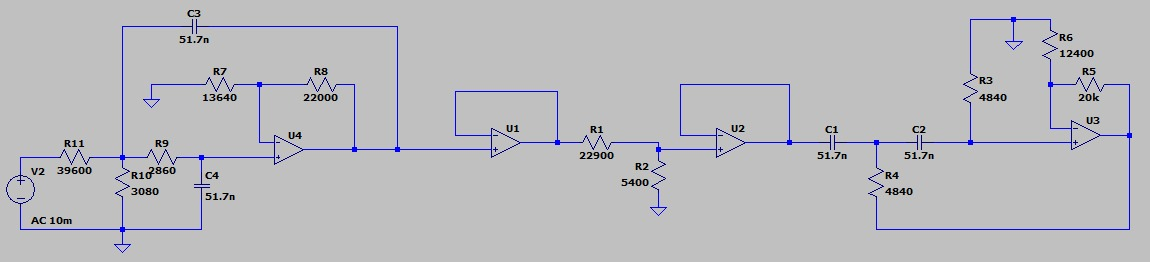
\includegraphics[width=1\linewidth]{Figura 14.jpg}
    \caption{Circuito del Peor Caso de la Desviación.}
\end{figure}

\begin{figure}[H]
    \centering
    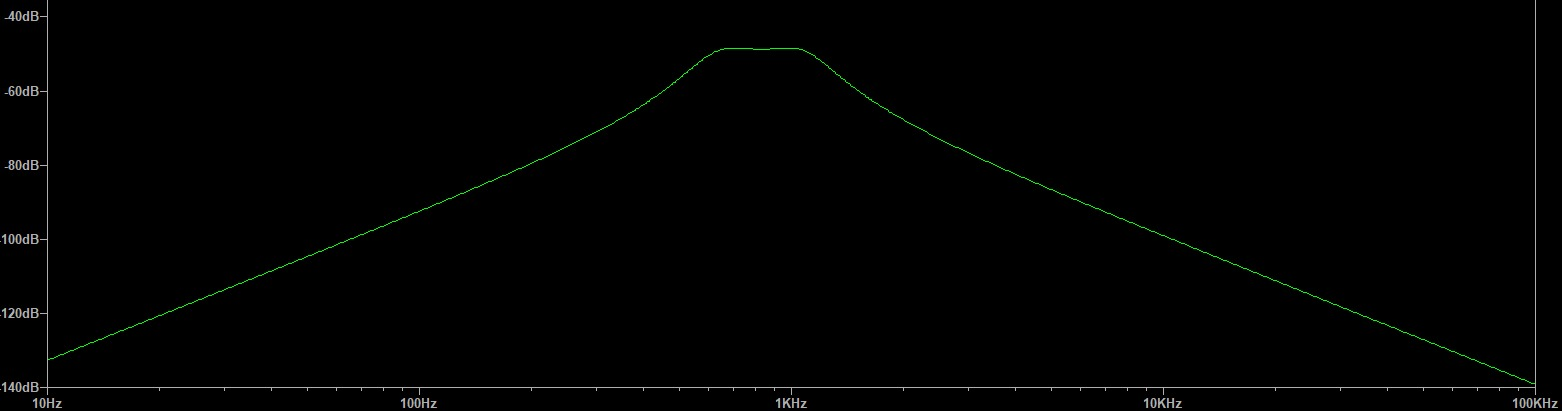
\includegraphics[width=1\linewidth]{Figura 15.jpg}
    \caption{Respuesta en Frecuencia del Peor Caso de la Desviación.}
\end{figure}

Se puede observar que el gráfico se desplazó un poco a la izquierda, lo que es coherente con el análisis previamente mencionado, puesto que al aumentar la resistencia y la capacitancia, se redujo la frecuencia central lo que quiere decir que el gráfico de módulo se desplazó a la izquierda. Numéricamente, implicaría que sí aumentara tanto $C$ como $R$ un $10 \ [\%]$, la frecuencia central del filtro ($\omega_o$) pasaría de $1001 \ [Hz]$ a $827 \ [Hz]$, como así que la frecuencia central del filtro pasa altos pasaría de $769 \ [Hz]$ a $636 \ [Hz]$ y la del pasa bajos de $1302 \ [Hz]$ a $1076 \ [Hz]$.

Analizando estos números, vemos que el: $\frac{\Delta \omega_{o}}{\omega_{o}}$  en porcentaje es de aproximadamente un: $17,38 \ [\%]$, la de: $\frac{\Delta \omega_{LP}}{\omega_{LP}}$ un: $17,35 \ [\%]$ y la de: $\frac{\Delta \omega_{HP}}{\omega_{HP}}$ un: $17,21 \ [\%]$.



\subsection{Simulación de Montecarlo}
De forma mas completa al análisis realizado en la sección anterior, podemos simular un variación del $10 \ [\%]$ de cada componente, simulando las tolerancias comerciales de componentes. A diferencia de la simulación realizada en el apartado anterior, aquí todo componente tiene la posibilidad de variar de un $0 \ [\%]$ a un $10 \ [\%]$ mientras que en el apartado anterior, todos los componentes aumentaron su tolerancia un $10 \ [\%]$ siguiendo una distribución dada por una Campana de Gauss la cual se evalúa un intervalo de confianza del $99,9 \ [\%]$ dado por $\sigma$ en el LTSpice. 

A continuación se presenta un diagrama esquemático del circuito al que se le realizará la simulación de Montecarlo:

\begin{figure}[H]
    \centering
    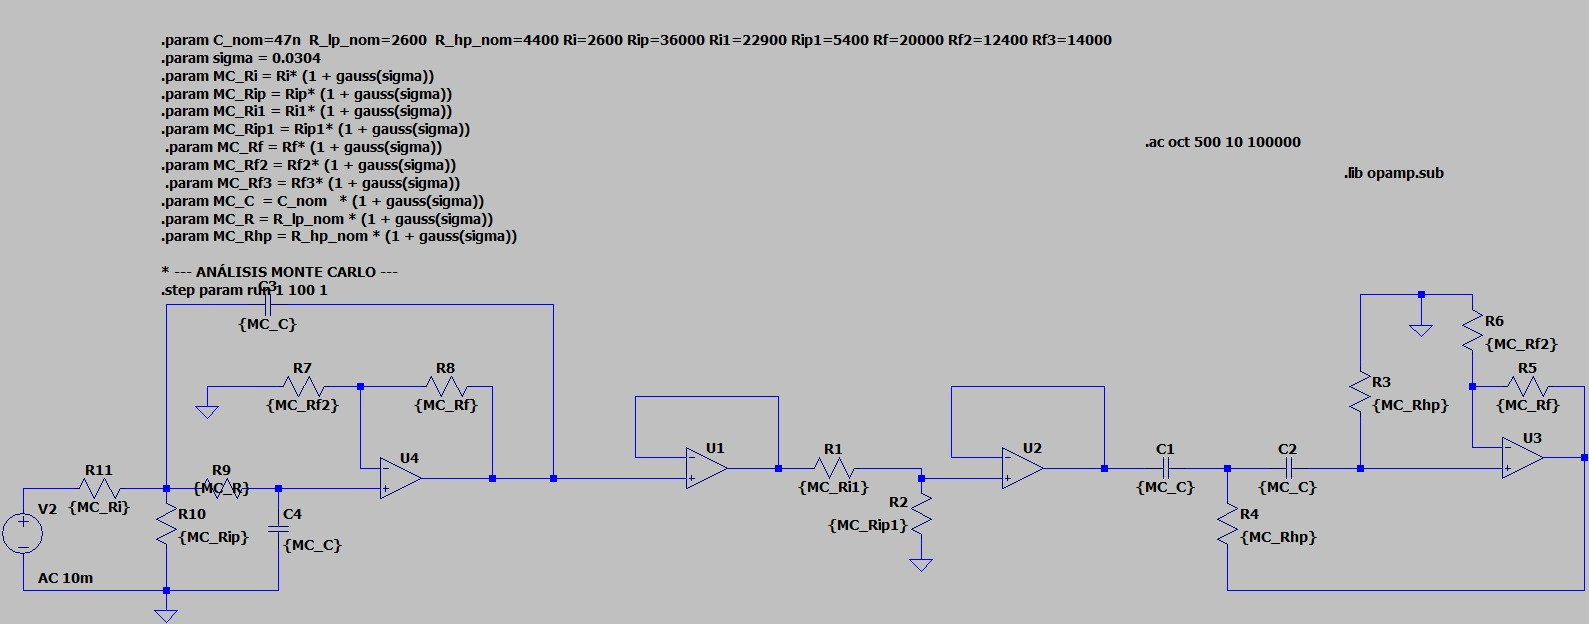
\includegraphics[width=1\linewidth]{Figura 16.jpg}
    \caption{Circuito final para simular.}
\end{figure}

El algoritmo para el cálculo de fuerza bruta se explica en la siguiente figura, donde se observa los distintos valores que se le atribuyen a los elementos de los circuitos y una función denominada $gauss()$, cuyo retorno es uno de los posibles valores dentro del intervalo de confianza correspondiente a la variable $\sigma$.

\begin{figure}[H]
    \centering
    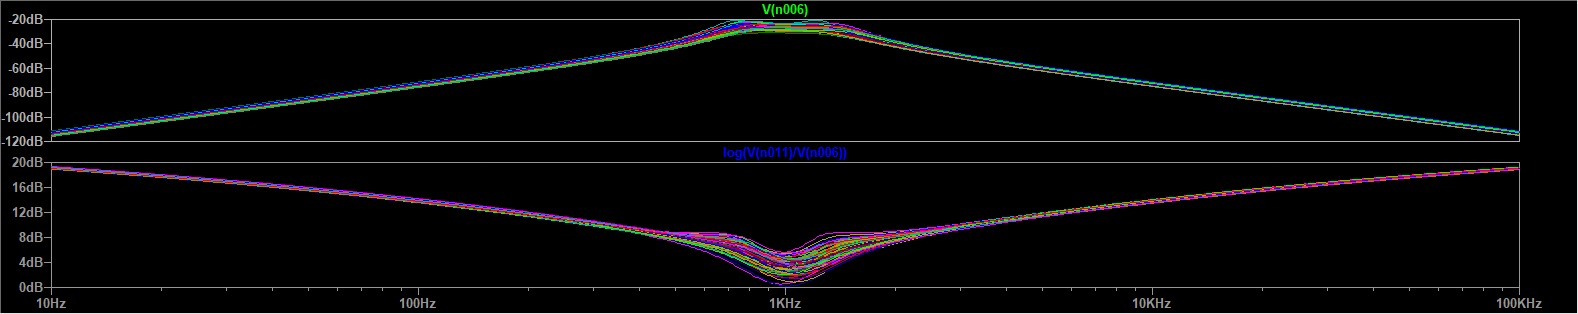
\includegraphics[width=1\linewidth]{Figura 17.jpg}
    \caption{Circuito de la Simulación Montecarlo de 100 pasos.}
\end{figure}

Realizando un pequeño ajuste de ganancia $k$ en el Filtro Pasa Altos ($r_{2} = 14 [k\Omega]$), se obtiene un comportamiento dinámico lo más similar posible al que menciona las especificaciones de la consigna par todas las simulaciones. A continuación se simula el sistema con el ajuste de ganancia mencionado y se observa el mejor cumplimiento de las especificaciones de la Figura 1:

\begin{figure}[H]
    \centering
    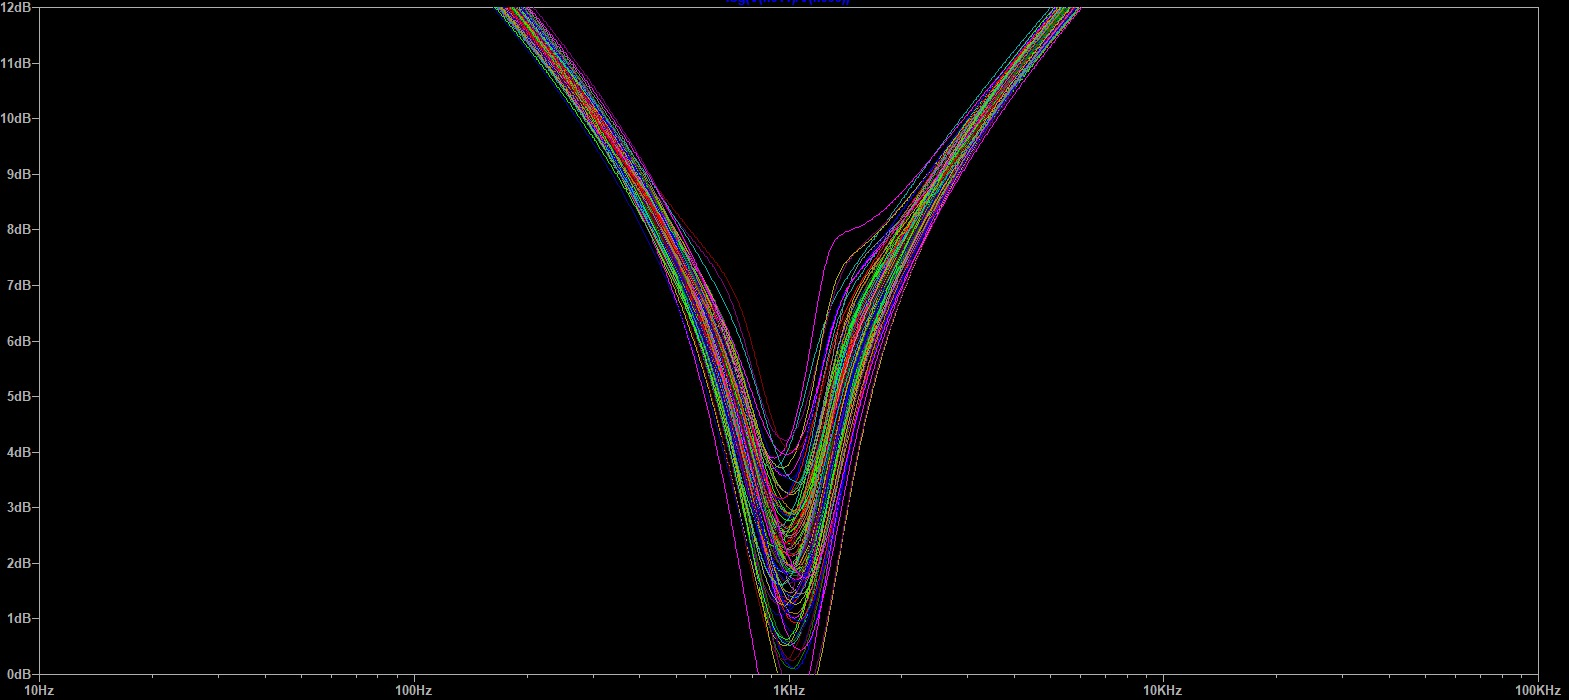
\includegraphics[width=1\linewidth]{Figura 18.jpg}
    \caption{Simulación Montecarlo final de 100 pasos.}
\end{figure}

\begin{figure}[H]
    \centering
    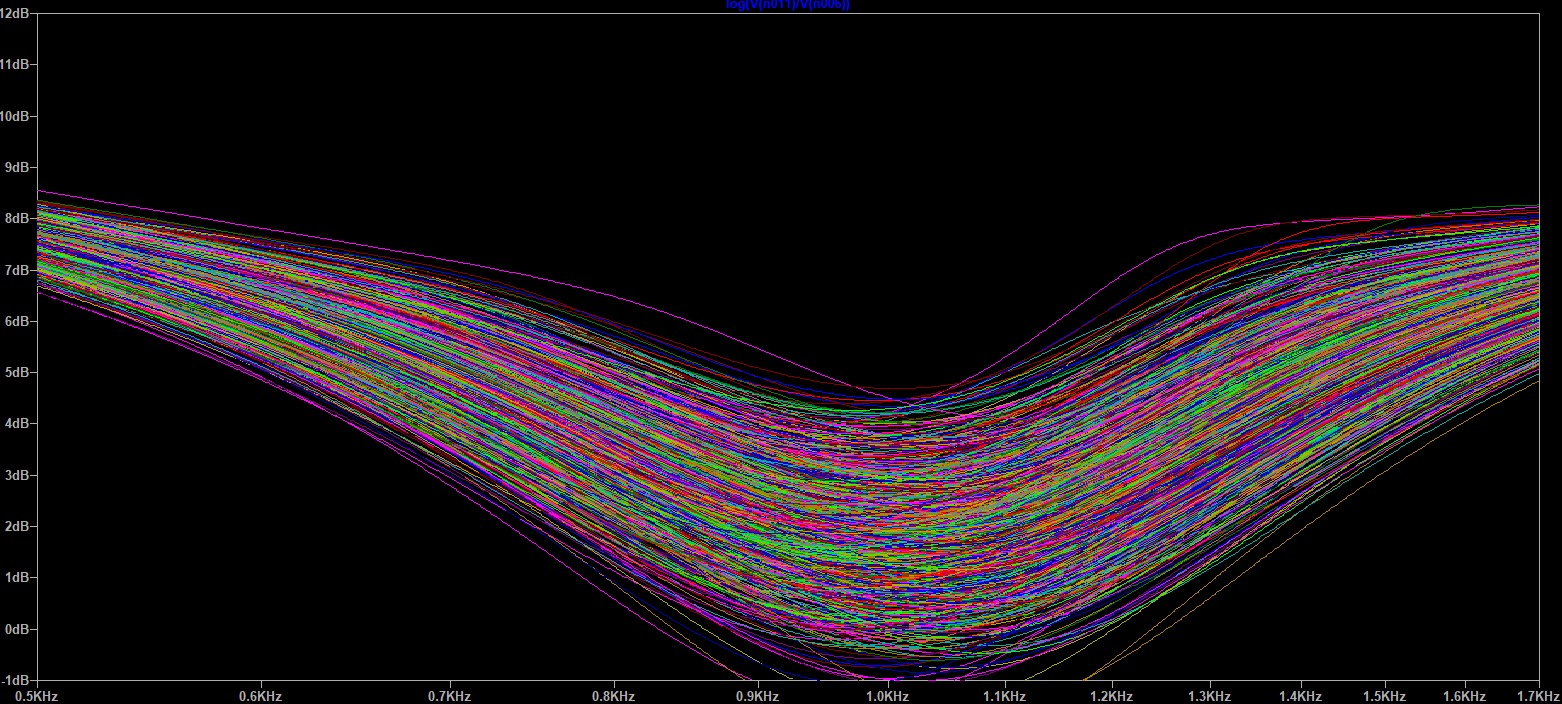
\includegraphics[width=1\linewidth]{Figura 19.jpg}
    \caption{Simulación Montecarlo final de 1000 pasos.}
\end{figure}



\section{Conclusión}
A lo largo de este trabajo se ha desarrollado un Filtro Pasa Banda, siguiendo los requerimientos presentados en la consigna. Partiendo de una aproximación en Matlab con los polinomios de Chebyshev hasta lograr sintetizar el filtro y realizar múltiples simulaciones respecto a su funcionamiento, tales como variaciones y tolerancias de los componentes como de su respuesta en frecuencia.



\section{Bibliografía}
\begin{itemize}
    \item \href{https://fcefyn.aulavirtual.unc.edu.ar/pluginfile.php/960585/mod_folder/content/0/%5BGobind_Daryanani%5D_Principles_of_Active_Network_Sy%28z-lib.org%29.pdf?forcedownload=1}{Principles of Active Network Synthesis and Design - G. Daryanani}
\end{itemize}



\section{Anexo}
A continuación se presenta el código en Matlab utilizado para obtener las funciones de transferencia de los filtros:

\begin{lstlisting}[style=matlab]
close all; clear all; clc;        % Trabajo Practico N°4 - Filtros Activos

%% Parametros de Entrada
fp = [800 1250];                  % Banda de Paso [Hz]
fs = [200 5000];                  % Banda de Rechazo [Hz]
Wp = 2*pi*fp;                     % Banda de Paso [rad/s]
Ws = 2*pi*fs;                     % Banda de Rechazo [rad/s]
Ap = 0.25;                        % Atenuacion maxima en Banda de Paso [dB]
As = 30;                          % Atenuacion minima en Banda de Rechazo [dB]

%% Calculo de FT
[n,Wp]    = cheb1ord(Wp,Ws,Ap,As,'s');
[num,den] = cheby1(n,Ap,Wp,'s');
Filtro    = tf(num,den)           % Funcion de transferencia calculada
[sos,g]   = tf2sos(num,den);      % Descomponemos en bicuadrativas

%% Implementacion como PasaAlto/PasaBajo
PasaBajo = tf(2*g*sos(1,1:3),sos(1,4:6))
PasaAlto = tf(1/2*sos(2,1:3),sos(2,4:6))

%% Graficos
figure; hold on;

%% Especificaciones Filtro
plot([fs(1)/10 fs(1) fs(1)],[-As -As -Ap],'Color','r','LineWidth',3);
plot([fs(2) fs(2) fs(2)*10],[-Ap -As -As],'Color','r','LineWidth',3);
plot([fp(1) fp(1) fp(2) fp(2)],[-As -Ap -Ap -As],'Color','g','LineWidth',3);

%% Filtro
h = bodeplot(Filtro);
p = getoptions(h);
p.PhaseVisible='off';
p.FreqUnits='Hz';
p.Grid='on';
setoptions(h,p);
bode(PasaBajo);
bode(PasaAlto);
\end{lstlisting}

\end{document}